\section{Lineare Gleichungssysteme}
		    \subsection{Matritzen und Vektoren}
			Matrix: $A = \begin{pmatrix}
				6&1&2\\
				5&4&0\\
				4&1&9
			\end{pmatrix}$ \qquad
			Einheitsmatrix: $E = \begin{pmatrix}
				1&0&0\\
				0&1&0\\
				0&0&1
			\end{pmatrix}$ \\
			\\
			Zeilenvektor: $a = \begin{pmatrix}
a_1&a_2&a_n \end{pmatrix}$ \quad Spaltenvektor: $b =  \begin{pmatrix} 1\\2\\3 \end{pmatrix}$ 	\\
			
			Standardbasisvektoren:  $ e_1=\begin{pmatrix}1\\0\\0\end{pmatrix},
\qquad
e_2=\begin{pmatrix}0\\1\\0\end{pmatrix},
\qquad
e_3=\begin{pmatrix}0\\0\\1\end{pmatrix}$ \\
	
				
			\subsection{Rechenregeln mit Matritzen und Vektoren}
		    \subsubsection{Addition / Subtraktion}
			Beschreibung für Spaltenvektoren $\rightarrow$ gilt analog für Zeilenvektoren! \\
			Beschreibung nur für Addition $\rightarrow$ gilt analog für Subtraktion! \\

			$a = \begin{pmatrix} 1\\2\\3 \end{pmatrix}$ \quad $b = \begin{pmatrix} 4\\5\\6 \end{pmatrix}$ \quad  $a+b = \begin{pmatrix} 1+4\\2+5\\3+6 \end{pmatrix}$ \\
			\\
			$A=\begin{pmatrix}
				1&2\\
				3&4\\
				5&6
			\end{pmatrix}$ \quad $ B=\begin{pmatrix}
				0&7\\
				5&3\\
				6&2
			\end{pmatrix}$ \quad $A+B=\begin{pmatrix}
				1+0&2+7\\
				3+5&4+3\\
				5+6&6+2
			\end{pmatrix}$

		    
			\subsubsection{Multiplikation}
			% Vektor mal Faktor
			$v = \begin{pmatrix} 1\\8\\4 \end{pmatrix}$ \qquad $\lambda \cdot v = \begin{pmatrix} \lambda \cdot 1\\\lambda \cdot 8\\\lambda \cdot 4 \end{pmatrix}$ \\
			\\
			
			%Matrix mal Faktor 
			$D=\begin{pmatrix}
				6&1&2\\
				5&4&0\\
				4&1&9
			\end{pmatrix}$ \qquad $\lambda \cdot 				D=\begin{pmatrix}
				\lambda \cdot 6 & \lambda \cdot 1 & \lambda \cdot 2 \\
				\lambda \cdot 5 & \lambda \cdot 4 & \lambda \cdot 0\\
				\lambda \cdot 4 & \lambda \cdot 1 & \lambda \cdot 9
			\end{pmatrix}$ \\
			\\
				
			% Matrix mal Vektor			

$D \cdot v = \begin{pmatrix}
\color{red}6&\color{red}1&\color{red}2\\
5&4&0\\
4&1&9
\end{pmatrix}
\begin{pmatrix}
\color{blue}1\\\color{blue}8\\\color{blue}4
\end{pmatrix}
=
\begin{pmatrix}
{\color{red}6}\cdot{\color{blue}1}+
{\color{red}1}\cdot{\color{blue}8}+
{\color{red}2}\cdot{\color{blue}4}
\\
5\cdot{\color{blue}1}+
4\cdot{\color{blue}8}+
0\cdot{\color{blue}4}
\\
4\cdot{\color{blue}1}+
1\cdot{\color{blue}8}+
9\cdot{\color{blue}4}
\end{pmatrix}
=\begin{pmatrix}
22\\37\\48
\end{pmatrix}$ \\
\\


			% Matrix mal Matrix
			$A=\begin{pmatrix}
\color{red}1&\color{red}2&\color{red}4\\
0&4&-1
\end{pmatrix}$, \qquad 
$B =\begin{pmatrix}
\color{blue}-2&4\\
\color{blue}-4&-5\\
\color{blue}2&4
\end{pmatrix}
\\
\\
A \cdot B =
\begin{pmatrix}
{\color{red}1}\cdot({\color{blue}-2})+{\color{red}2}\cdot({\color{blue}-4})+{\color{red}4}\cdot{\color{blue}2} &
{\color{red}1}\cdot 4+{\color{red}2}\cdot(-5)+{\color{red}4}\cdot 4\\
0\cdot ({\color{blue}-2})+4\cdot({\color{blue}-4})+(-1)\cdot {\color{blue}2} &
0\cdot 4+4\cdot(-5)+(-1)\cdot 4
\end{pmatrix}$ \\


			\subsubsection{Division}
			Divisionen von Matritzen werden durch eine Multiplikation mit der inversen Matrix durchgeführt.

   			\subsubsection{Zusammenfassung / Erweiterung der Rechenregeln}
   			\begin{tabular}{lll}
   			Symmetrie: & $ A = A^t$ \\   			
   			Orthagonalität: &  $ A A^t = A^t A = E $  & $A^{-1} = A^t$\\
   			& $A^t$ auch orthagonal & $\det(A) = \pm 1$ \\
   			Produkte: & \textbf{AB $\neq$ BA} & $(AB)C = A(BC)$\\
   			& $EA = A = AE$  & $A(B + C) = AB + AC$\\
   			& $A (\lambda B) = (\lambda A) B$ & \\
   			Transponiert: & $(AB)^t = B^t A^t $ \\
   			Inverse: & $A^{-1} A = E$ & $(AB)^{-1} = B^{-1} A^{-1} $ \\
   			Potenzen: & $(A^t)^{-1} = (A^{-1})^t $ \\
   			\end{tabular}
		    
		    
		    \subsection{Tranponierte Matrix $A^t$}
		    Spiegelung an Diagonalen \\
		    \\
		    $A=\begin{pmatrix}
				a&b&c\\
				d&e&f\\
				g&h&i
			\end{pmatrix}$ \quad $ A^T =\begin{pmatrix}
				a&d&g\\
				b&e&h\\
				c&f&i
			\end{pmatrix}$    
		        
		        
		    \subsection{Inverse Matrix $A^{-1}$}
		    Die Inverse Matrix ist \textbf{nur für quadratische Matritzen} definiert.
		    Die Inverse Matrix kann durch dar Gauss-Verfahren oder mit dem Entwicklungssatz berechnet werden. \\
		    \\
		    1. Gauss: \quad $A^{-1}$ \quad \begin{tabular}{|c|c|}
		    					\hline
		    					A & E \\
		    					\hline
		    					\end{tabular} \quad $\underrightarrow{\text{Gauss}}$ \quad \begin{tabular}{|c|c|}
		    					\hline
		    					E & $A^{-1}$ \\
		    					\hline
		    					\end{tabular} \\
					\\
			2. Entwicklungssatz: \quad $A^{-1} = \frac{1}{\det(A)} \cdot \mathrm{adj}(A) $  für $\det(A) \neq 0$ \\
			\\
			Bsp. 2 x 2 Matritzen: \quad $A^{-1} = \frac{1}{ad-bc} \cdot \begin{pmatrix}
			d & -b \\
			-c & a 
			\end{pmatrix} $  für $\det(A) \neq 0$ \\
			\\
			\textbf{$\rightarrow$ für Variante Entwicklungssatz siehe Beispiel nächste Seite} \\
			

			\subsection{Lineares Gleichungssystem }
			 Ein Lineares Gleichungssystem kann als Matrix geschrieben werden:
			 
			 \subsubsection{Beispiel}
			 \begin{tabular}{llllll |c c | c|}
			 $x$ & + & $3 \, y$ & = & $1$  \\
			 $-x$ & + & $5 \, y$ & = & $-1$  \\
			 \end{tabular} 
			\\
			 
			Das Gleichungssystem wird in eine Matrix abgefüllt: \\
			\\
			 \begin{tabular}[h]{|c c | c|}
			 \hline
			 $x$ & $y$ & $b$\\
			 \hline
			 $1$ & $3$ & $1$ \\
			 $-1$ & $5$ & $-1$ \\
			 \hline
			 \end{tabular}
			 
			 
			 \subsubsection{Lineare Gleichungssysteme lösen}
			 \begin{tabular}{ll}
			 $\bullet$ & Gauss-Algorithmus \\
			 $\bullet$ & Inverse Matrix $x = A^{-1} \cdot b$ \\
			 $\bullet$ & Cramersche Regel \\
			 \end{tabular}
			 
			 
		    \subsection{Gauss-Algorithmus}
		    Die aktuelle Zeile wird durch das \textcolor{red}{Pivot-Element} ($\neq 0$) geteilt. \\  
		     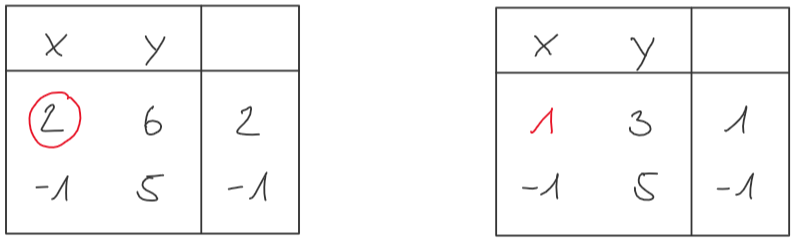
\includegraphics[width=0.45\linewidth]{Bilder/gauss1} \\
		   	

		    Anschliessend werden alle Spalten unterhalb des Pivots auf \textcolor{blue}0 gesetzt, indem man das x-Fache der neuen "Pivot- Zeile" von der entsprechenden Zeile subtrahiert / addiert. \\
		    \\
		    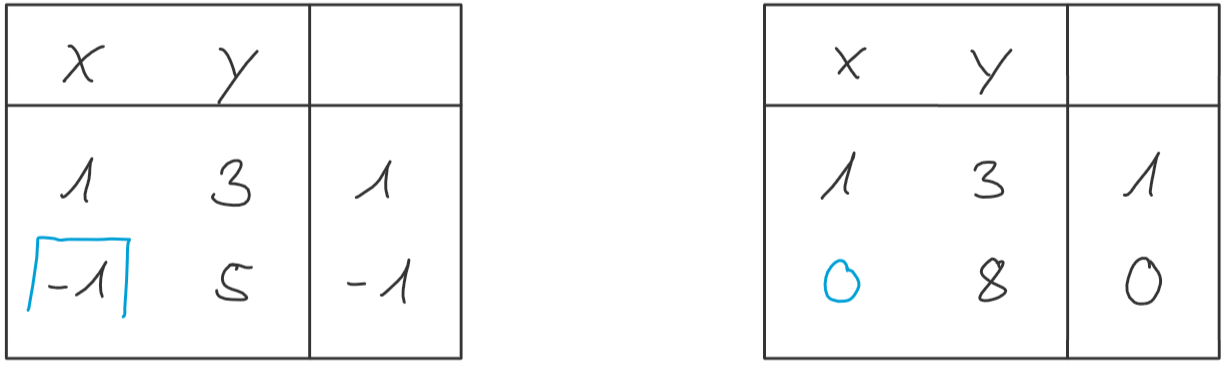
\includegraphics[width=0.45\linewidth]{Bilder/gauss2} \\
		    \\
		    Schritt 1 und Schritt 2 wiederholen, bis nur noch 1en auf der Diagonalen stehen. \\
		    \\
		    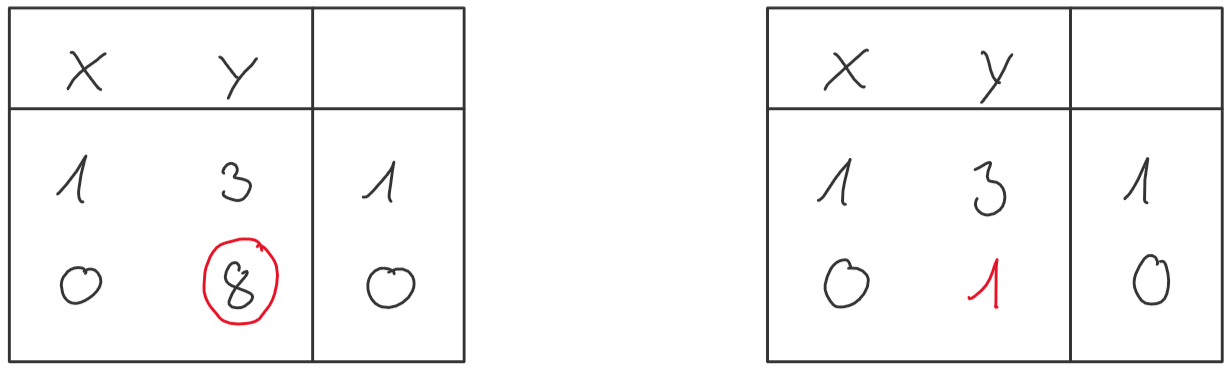
\includegraphics[width=0.45\linewidth]{Bilder/gauss3} \\
		    \\
		    Wenn nur noch 1en auf der Diagonale stehen muss nur doch die blaue Operation durchgeführt werden (Rückwärts-Einsetzen) \\
		    \\
		    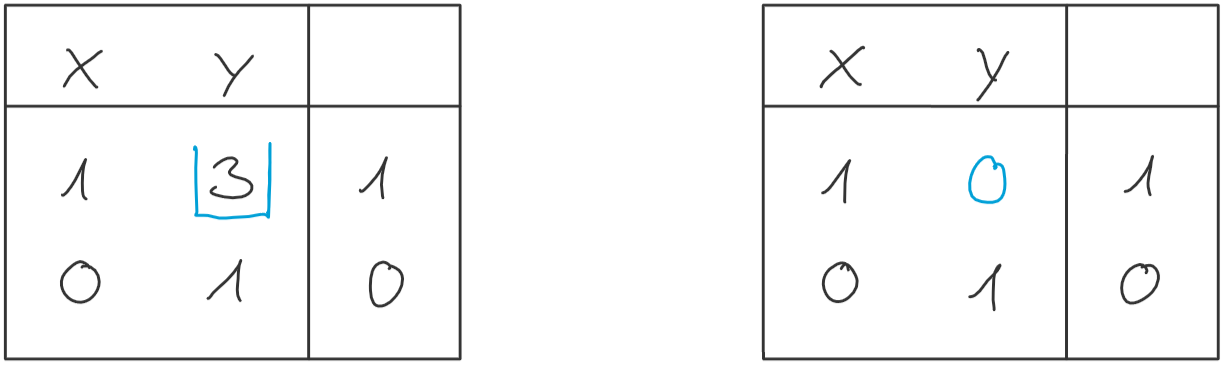
\includegraphics[width=0.45\linewidth]{Bilder/gauss4} \\
		    
		    
		    
			\subsubsection{Spezialfall RREF}
	
			\begin{minipage}[b]{.5\linewidth} 
  			\includegraphics[width=\linewidth]{Bilder/RREF-Tableau}
			\end{minipage}
			\hfill
			\begin{minipage}[b]{.45\linewidth} 
  			Wenn die nächste Spalte im Gauss-Algorithmus kein Pivot-Element enthält (0 ist), kann die Spalte 						übersprungen werden. Die Spalte repräsentiert eine 					\textcolor{green}{frei wählbare Variable} \\
			$\rightarrow$ Siehe Abschnitt zu Lösungsmenge\\	
			\end{minipage}			
   		
   			
   			\vfill\null
   			\columnbreak
   		
   		
   		
   		
		    \subsubsection{Simulatane Lösung (mehrere Rechte Seiten)}
		    Wenn zwei Gleichungssysteme sich nur auf der rechten Seite \\
		    unterscheiden können sie in das gleiche Gauss-Tableau abgefüllt werden.\\
		    $\rightarrow$ normal mit Gauss-Algorithmus lösen \\
		    \\
		    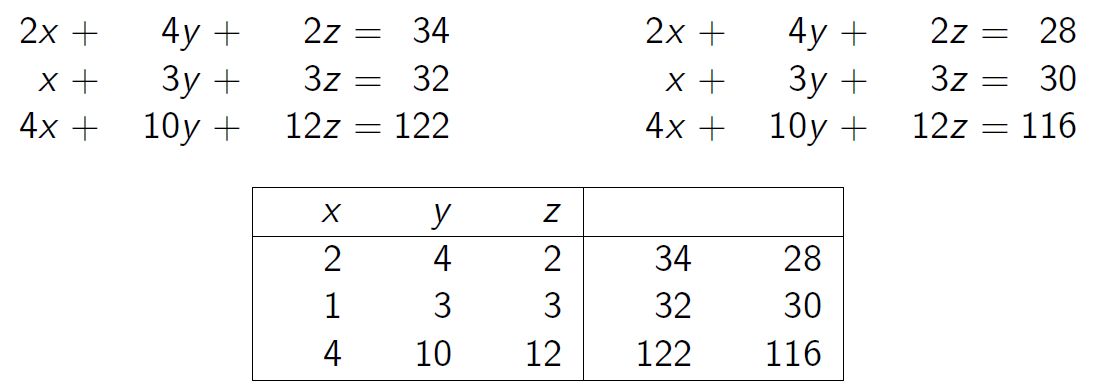
\includegraphics[width=0.6\linewidth]{Bilder/mehrere_rechte_seiten}
		    
		    
		    \subsection{Lösungsmenge}
		    	Falls mehr Unbekannte als Gleichungen vorhanden sind, können nicht alle Unbekannten bestimmt werden. \\
		    	

		 	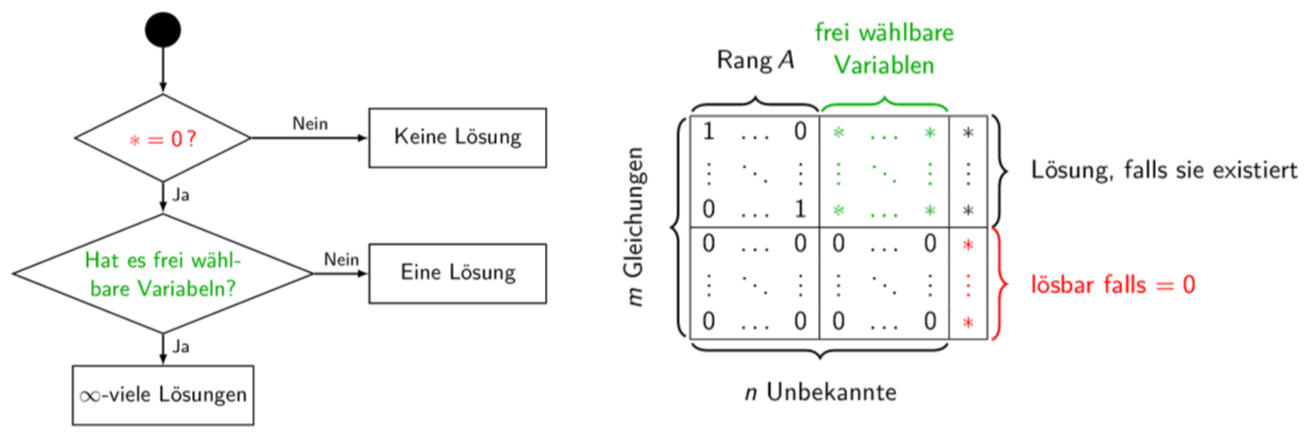
\includegraphics[width=0.9\linewidth]{Bilder/entscheidungsbaum} 	\\
			 \\
			 Wenn es unendlich viele Lösungen gibt kann die Lösungsmenge folgendermassen angegeben werden \\
			 \textbf{Vorzeichenwechsel bei frei wählbaren Variablen beachten!}\\
			 \\
			  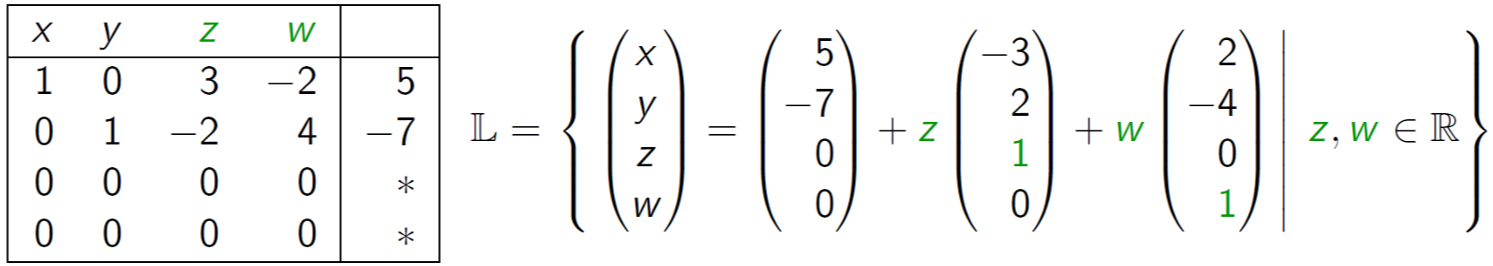
\includegraphics[width=0.9\linewidth]{Bilder/loesungsmenge-gauss-tableau} \\
				  
		    
		    \subsection{Rang einer Matrix}
			Anzahl linear unabhängiger Zeilen / Spalten \\		    
		    Entspricht der Anzahl eindeutig bestimmbarer Variablen \\
		    
		    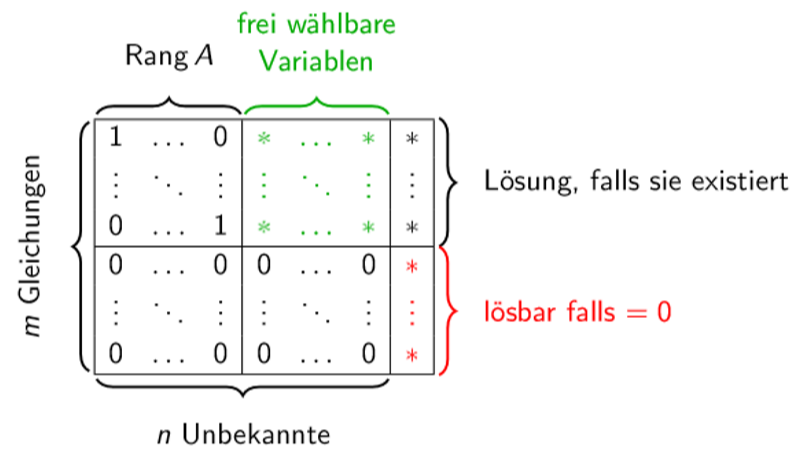
\includegraphics[width=0.7\linewidth]{Bilder/loesungsmenge-gauss}
		    
			
			\vfill\null
			\columnbreak		    
		    
		    
		    
		    \subsection{Lineare Abhängigkeit}
		    Wenn eine Zeile ein Vielfaches einer anderen Zeile ist, sind die Zeilen linar abhängig. \\
		    Beim Gauss-Algorithmus entsteht eine Nullzeile. \\
		    \\
		    $\lambda_1 \cdot$ Zeile 1 + $\lambda_2 \cdot$ Zeile 2 + $\lambda_3 \cdot$ Zeile 3 = Nullzeile \\
		    \\
		    Um die Koeffizienten $\lambda_i$ zu finden wird dir ursprüngliche \\
		    Matrix A transponiert und auf Null gesetzt. \\
		    \\
		    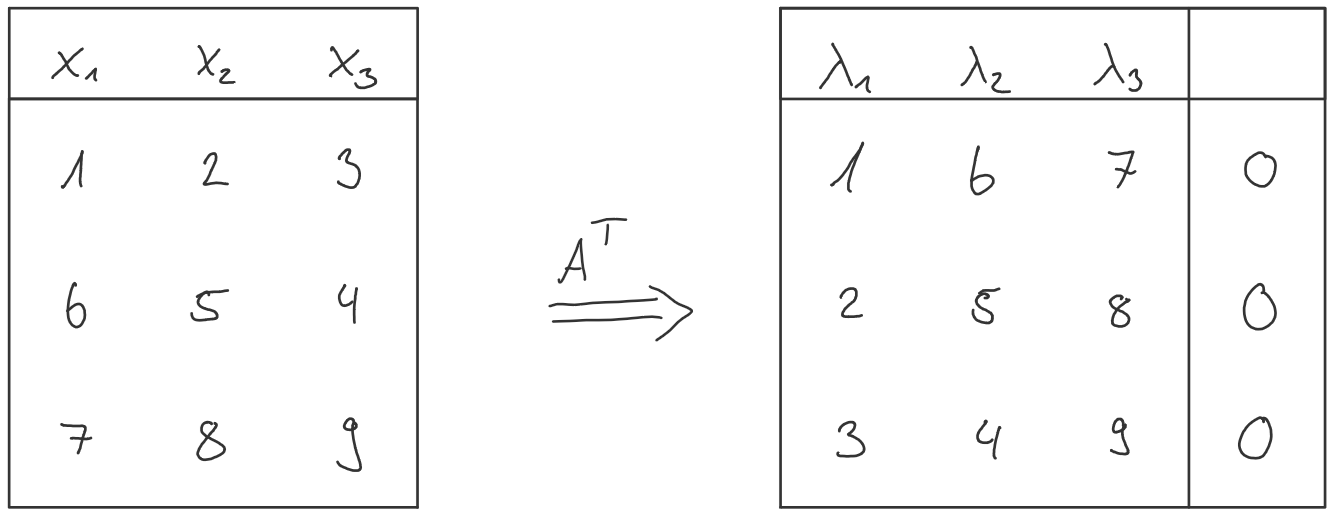
\includegraphics[width=0.5\linewidth]{Bilder/lineare-abhaengigkeit_1} \\
		    \\
		    Die neue Matrix wird mit dem Gauss-Verfahren gelöst\\
		    
		    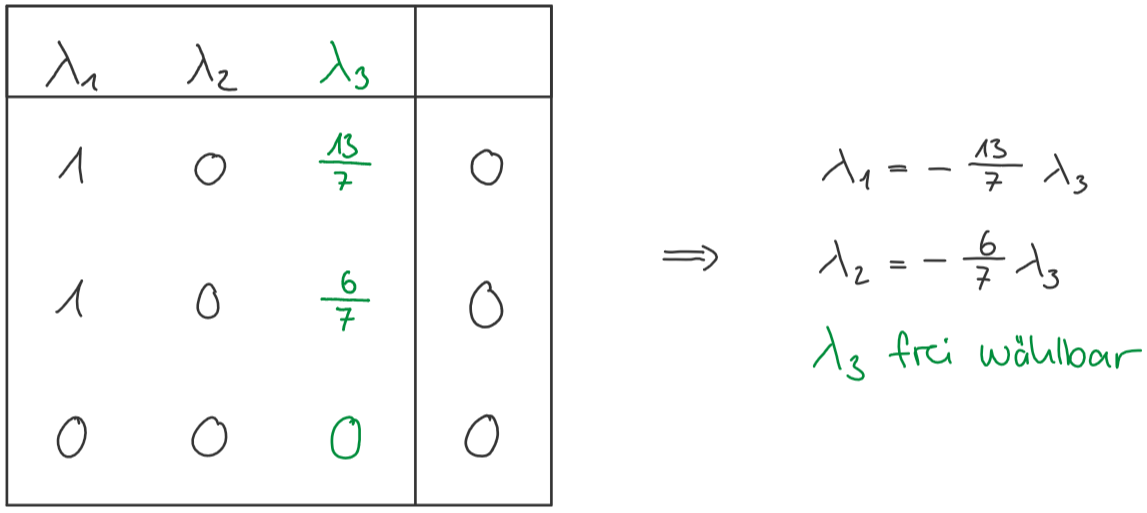
\includegraphics[width=0.5\linewidth]{Bilder/lineare-abhaengigkeit_2} \\
		    
		    
		    
			\subsection{Lineares Gleichungssystem $A \cdot x = b$}	
			Ein lineares Gleichungssystem entstspricht dem Produkt aus Matrix mal Vektor \\
			\\
			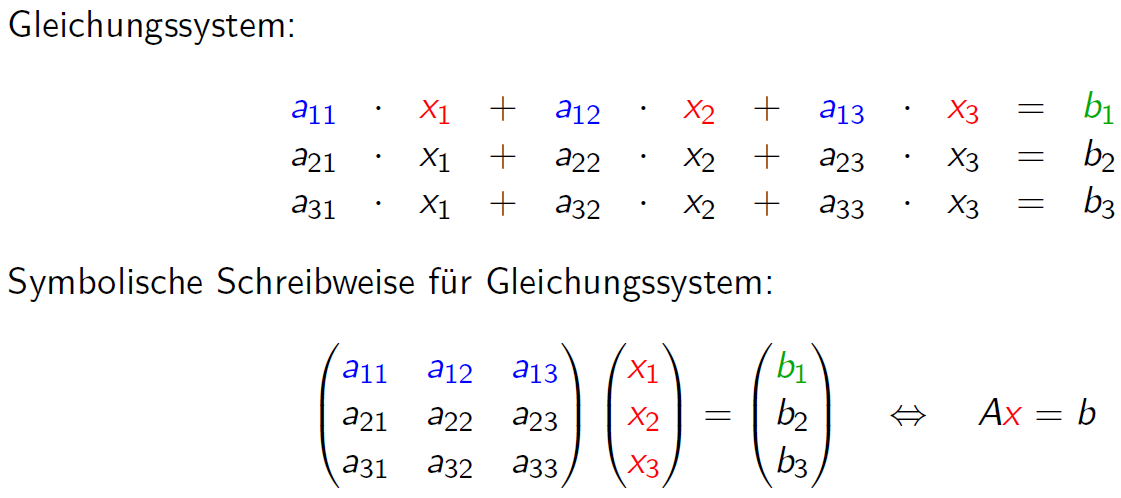
\includegraphics[width=0.8\linewidth]{Bilder/Ax_b} \\
			\\
			Dieses Gleichungssystem bestitz die Lösung $x = A^{-1} \cdot b$ \\	
				    
		    
		    
		    \subsection{Homogene / Inhomogene LGS}
		    \begin{tabular}{ll}
		    Inhomogen: & $Ax = b$ \\
		    Homogen: & $Ax = 0$ \\
		    \end{tabular}
		    
		    
		    
		    \subsection{Reguläre / Singuläre Matrix}
		    Die Begriffe sind nur für quadratische Matritzen definiert! \\
		    \begin{tabular}{lll}
		    regulär: & genau 1 Lösung & $\rightarrow$ det(A) $\neq$ 0 \\
		    singulär: & 0 oder $\infty$ Lösungen & $\rightarrow$ det(A) = 0 \\
		    \end{tabular}
		    
		    \vfill\null
		    \columnbreak
		    